\documentclass[a4paper, oneside, 10pt]{article}
\usepackage{float}
\usepackage{amsfonts} % if you want blackboard bold symbols e.g. for real numbers
\usepackage{graphicx} % if you want to include jpeg or pdf pictures
\usepackage{listings} % entering code.

\graphicspath{{images/}}

\title{{\bf 15-869 Visual Computing System Final Project Report \\
 \large Solving Out of Core Ray Tracing Problem by a Distributed Path Tracing System}} % change this

\author{Xiao Li (xiaol2) and Yihua Eric Fang (yihuaf)}

\date{\today} % change this

\begin{document}

%%%%%%%%%% PRELIMINARY MATERIAL %%%%%%%%%%
\maketitle
\thispagestyle{empty}
\newpage
\begin{center}
\vspace*{\fill}
\section*{Abstract}
Parallel Breadth-First Search, from the past to present.\\
\vspace*{\fill}
\newpage
\end{center}

\tableofcontents
\newpage

%%%%%%%%%% MAIN TEXT STARTS HERE %%%%%%%%%%
\section{Introduction}
\section{Background}
\paragraph{} In general, the renderers used in animation, film or FX industries could be categorized as on-core and out-of-core renderers.  In the context of ray tracer, on core ray tracer ensures the whole scene to render fits in the DRAM of a machine. This allows the ray tracer to generate random numbers of rays when intersection happens, and trace them without worrying about scheduling the loading and unloading scenes. 

\paragraph{} Out-of-core renderers, on the other hand, assumes the scenes are too big to fit in the DRAM of a single machine. One of the major benefits of out-of-core renderers is they have no hard upper limits on geometries to render. However, usually the out-of-core renderers need to take extra efforts for scheduling the ray tracing system, manage the geometries workload balancing across machines, perform extra work reduction, optimization of memory coherence and hide all kinds of communication latency. 

\paragraph{} We designed a system to perform out-of-core rendering, based on Azurender, a ray tracing based renderer. We designed and implemented two algorithms. Different from the design of Hyperion or Pantaray, which are more focused on smarter sorting, loading and unloading of rays, ray packets or BVHs to hide the latency caused by hard disk accessing, our design load the scenes into DRAMs in a distributed system and focus on the scheduling and optimization for inter-machine communications. 

\section{System Design}
\subsection{System Overview}
\subsubsection{Ray Tracing System}
\paragraph{} Our system involves a basic ray tracing logic, as shown in the $Figure 1$. Like any other ray tracing system, if we do not generate second rays at all, it would have direct illumination only. For simplicity, we assumed all second rays intersection would be a lambertian diffusive surface hit.
\begin{figure}[h]
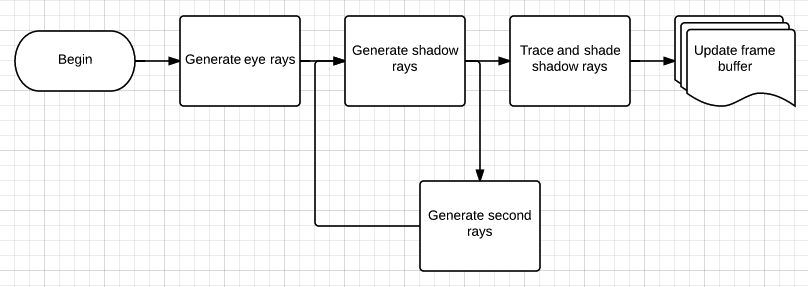
\includegraphics[width=\textwidth] {img1}
$Figure. 1\ Ray\ tracing\ system\ overview$
\end{figure}
\subsubsection{Distribution Policy}
\paragraph{}The distribution of scene is shown in figure $Figure. 2$. We tested the system on CMU’s gates center computer clusters that use AFS file system. Our scene file, a xml description file indicates the distribution policy of geometries in the scene. At this stage, we manually distribute the geometries, but there is the potential of automatic and smart distribution of geometries. We used Open MPI message passing interface for data flow control.
\begin{figure}[h]
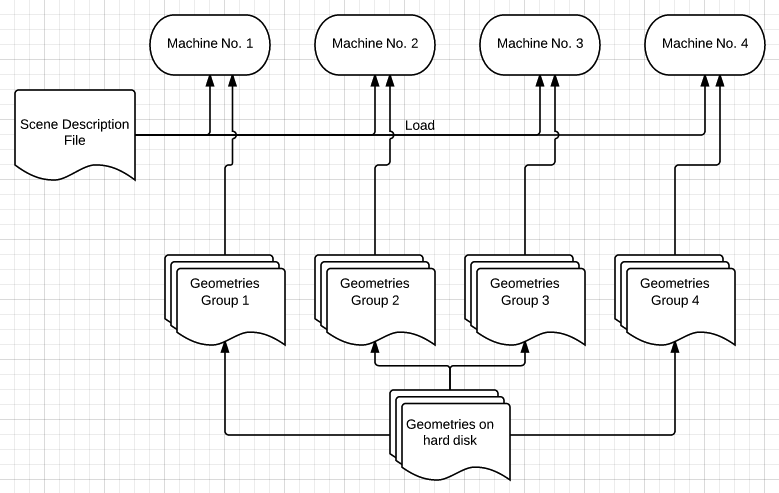
\includegraphics[width=\textwidth] {img2}
$Figure. 2\ System\ distribution\ policy$
\end{figure}

\subsection{Approach 1 - Staged}
\subsubsection{Overview}
\paragraph{}The first approach is a stage by stage algorithm. The idea behind it is to take the advantage of distributed machines across the network. Each of the ray tracing stage is separated. Each of the nodes (machines) in the system performs the exact same operations at the same stage. After each stage, there would be a synchronized blocking communication in between machines for exchanging the required data for next stage. The data would be duplicated across machines. For example, if one eye ray hits multiple root level bounding boxes of different nodes, the eye ray would be duplicated and sent to multiple machines. 
After the stage of tracing and when comes to the stage of shading, each machine / node would update their own local frame buffer, depth buffer and shadow map. Then a gather operations is performed on root node, and framebuffer information from different nodes would be merged.
The system is shown in $Figure 3$.
\begin{figure}[h]
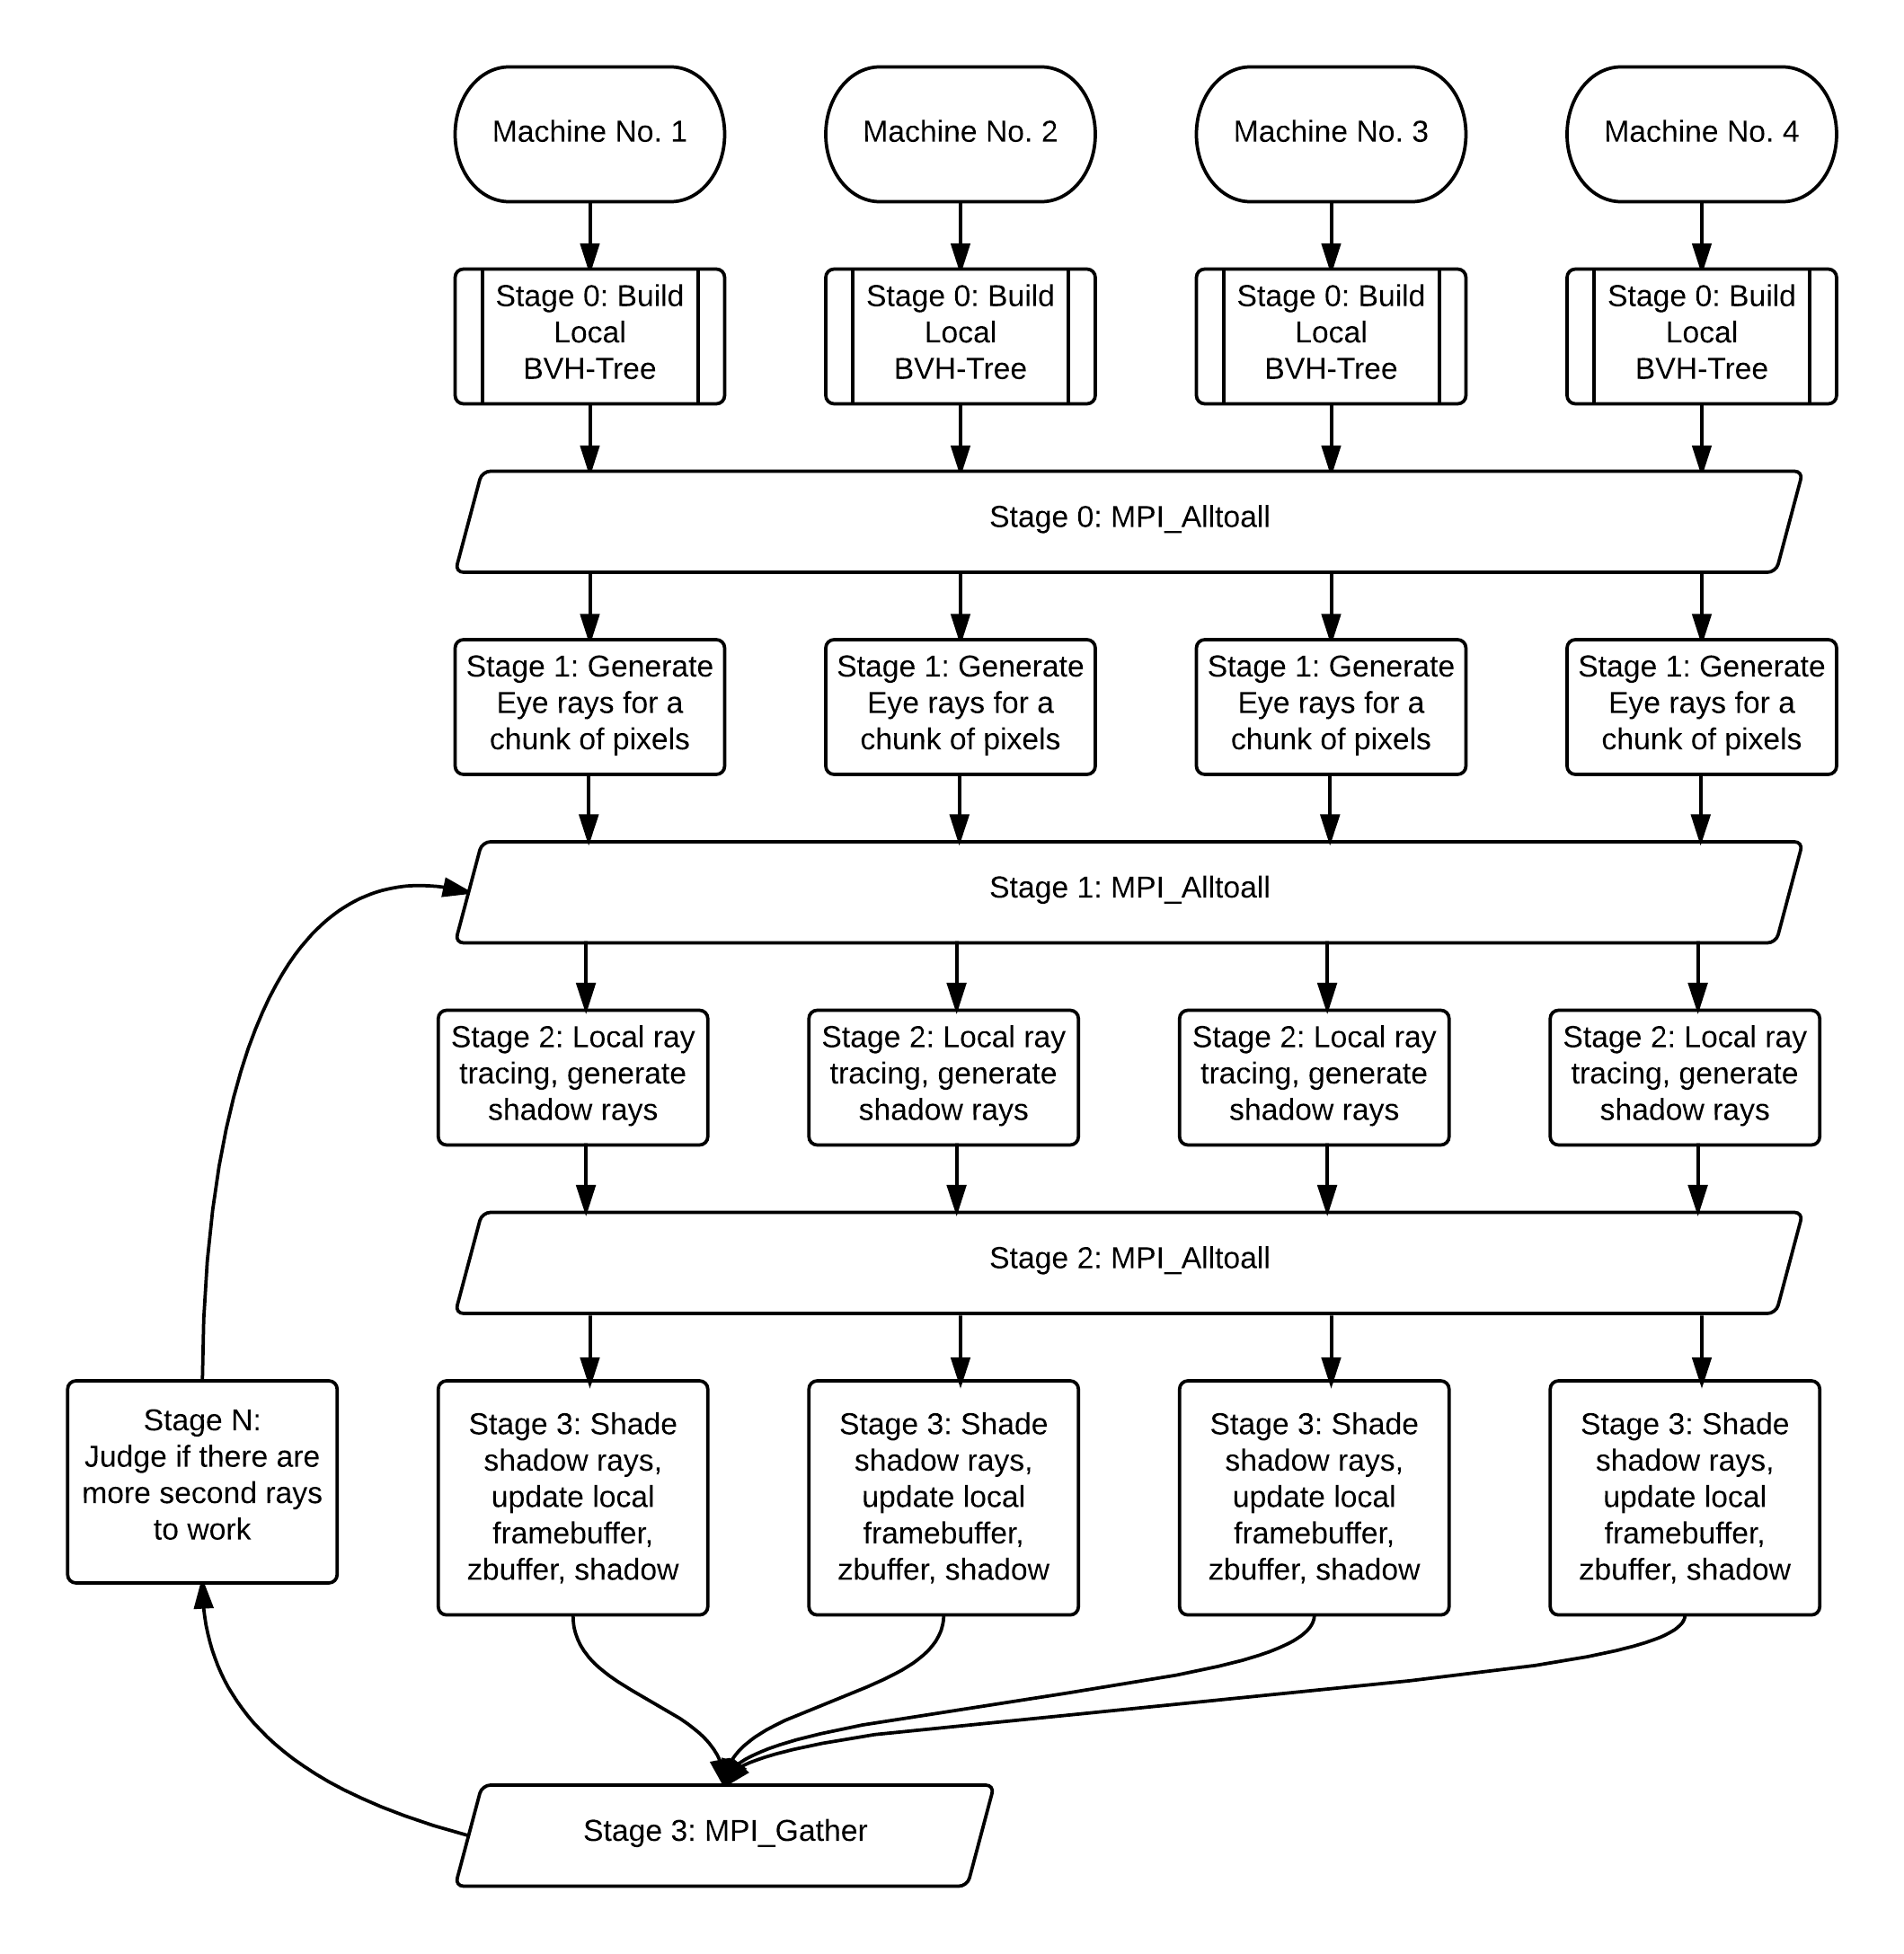
\includegraphics[width=\textwidth]{algo1}
$Figure. 3\ Algorithm 1.\ Workflow\ of\ staged\ system$
\end{figure}
\paragraph{}The assumption behind it is that local ray tracing and shading is fast and cheap and inter-nodes communication is expensive, meanwhile, Open MPI is optimized for large chunk of data exchange. The design assumes that the overhead of increased replicated work is lower than the overhead of increased communication.
\subsubsection{Work Flow}
\paragraph{}The pseudocode is as following, at the end of each function, there would a data exchange with synchronized blocking message passing:
\lstset{language=c++}
\begin{lstlisting}[frame=single]
    void mpiTrace()
    {
        mpiStageDistributeEyeRays();
        mpiAllToAllExchange(eyerays);
        
        mpiStageLocalRayTracing(eyerays);
        mpiAllToAllExchange(shadowrays);
        mpiAllToAllExchange(secondrays);
        
        mpiStageShadowRayTracing(shadowrays);
        mpiGather(framebuffer, root);
       	mpiMergeFrameBuffer();
        
        while (second rays are not done) {
            mpiStageLocalRayTracing(second rays);
            mpiAllToAllExchange(shadowrays);
            mpiAllToAllExchange(secondrays);
            
            mpiStageShadowRayTracing(shadowrays);
            mpiGather(framebuffer, root);
            
            mpiMergeFrameBuffer();
        }
    }
\end{lstlisting}
$Algorithm. 1\ Synchronized\ staged\ based\ path\ tracing$
\subsubsection{Algorithm Discussion}
\paragraph{} The core idea behind the algorithm is to minimize node-to-node communication. Note that the goal is to diminish communication frequency, instead of diminish the communication size. The algorithm would send all rays to all nodes that potentially have an intersection with the rays in the ray list. The sending and receiving of ray data always happen at the same time for all nodes. Once every node gets the ray data needed for ray tracing, it would immediately do local ray tracing, and generate more rays needed for the next stage. 
\paragraph{} Apparently, a major drawback is the duplication of work. Imaging a ray hits the bounding boxes of all nodes, the concept ray would be duplicated and sent to all nodes, each node would do a local tracing and shading, whereas at the final merging stage, there should be only one shading result needed. Therefore for each ray that is sent to $N$ nodes, $N-1$ works are wasted. The ratio of wasted work depends on how many nodes each ray might potentially hit. However, the worst case scenario is all nodes' geometries occupy the whole screen space, and each ray must hits all nodes. This would cause the system to be running as nodes numbers $(N)$ of independent ray tracer, each one has $1/N$ total geometries, plus inter communication overhead. Given the fact that our ray tracer runs reasonably fast on local ray tracing, the performance would not be so bad at first glance.
\paragraph{}However, the second rays could cause further problems since second rays might explode if duplicated works are not reduced. Assuming each first ray hit would generate $m$ more second rays, and each ray would on average hits $n$ geometries, and recursion depth is $k$. For a regular ray tracer, a ray hit would in total cause $m^k$ ray testing, our first algorithm would cause $(n*m)^k$ rays. The increase of workload would be proportional to $n^k$. This would become a disaster if $n$ increases, therefore we expect a relatively bad scalability to this system.
\subsubsection{Future Optimization}

\paragraph{}The problem mentioned in last section however is not completely unsolvable. An optimization might be perform a $MPI\_Scatter$ after $MPI\_Gather$ after the root node merged the buffer information from all nodes. If root node is able to send the depth buffer information back to all nodes, each node would be able to update its next step ray data list and discard all the works they don't need to do. This would take just one additional synchronized communication and reduce the scale factor from $n^k$ down to 1.

\subsection{Approach 2 - Asynchronous}
\subsubsection{Overview}

\subsubsection{The Ray Request}
\paragraph{} Before explaining how master and slaves processing each rays, we want to explain the data in the ray struct.  For simplicity, we used the ray struct that was already defined in the single thread ray tracer as requests in the system.  The struct contains the ray information such as its starting point, direction and etc. with extra header information needed by the system.  Below is the definition of the ray struct.
\lstset{language=C++} 
\begin{lstlisting}[frame=single] 
struct Ray
    {
    // Ray Info:
        Vector3 e;  // Ray starting point
        Vector3 d;  // Ray direction
 
        Color3 color; // Result color
        
        float mint, maxt, time;  // t values
        int x, y;  // location
        int depth;  // Ray depth
        
    // Extra Header information needed for the system:
        ERayType type;  // Ray type
        bool isHit;  // Did the ray hit a surface
        Vector3 hit;  // Hit point if hit
        Vector3 hitNormal;  // Hit point's normal
    }; 
\end{lstlisting}
\paragraph{} The first info we need in the header is the ray type, which we use to distinguish rays arrived from other node. There are four different kinds of rays in the system.
\begin{enumerate}
\item Eye Ray (ERayType$\_$Eye)
\item Shadow Ray (ERayType$\_$Shadow)
\item Global Illumination Ray (ERayType$\_$GI)
\item Global Illumination Shadow Ray (ERayType$\_$GIShadow)
\end{enumerate}
\paragraph{} The other info we need in the header are if the ray hit a surface or not and if hit the hit point and hit point normal associated.\\ 
\subsubsection{Slave Processing Rays}
\paragraph{} For an easier explanation, we will start with slaves' operations to process rays.  Below is the pseudo specifying the slaves' operations.
\begin{lstlisting}[frame=single] 
case ERayType_Eye:
case ERayType_GI:
{
  int next_node;
  next_node = localRaytrace(ray);
  if (next_node == root && ray.isHit)
  {
    // generate shadow ray
    // check bounding box
    // push result list
    generateShadowRay(ray, shadowRay);
    next_node = checkNextBoundingBox(shadowRay, root);
    result_list.push_back(next_node, shadowRay);

    if (ray.depth > 0)
    {
      generateGIRay(ray, giRay);
      next_node = checkNextBoundingBox(giRay, root);
      result_list.push_back(next_node, giRay);
    }
  }
  else {
    result_list.push_back(next_node, ray);
  }
}
break;
case ERayType_Shadow:
case ERayType_GIShadow:
{
  int next_node = localRaytrace(ray);
  result_list.push_back(next_node, ray);
}
break;
\end{lstlisting}

\paragraph{} If the slave received eye ray or a global illumination ray, the slave would first locally trace the the ray on the models on this slave node. After the trace, it would check the ray against all the node bounding boxes to determine the who is responsible for processing this node next. Later, we will discuss the algorithm used to determine the next node in details.  If the node hit the model on the slave and there are no more slave node that intersects with this ray, the slave will generate a shadow ray and a global illumination ray if the ray has not reached the depth yet. Otherwise, the slave would sent the eye ray or the global illumination ray to the next node responsible for processing.

\paragraph{} If the slave received a shadow ray from eye ray or global illumination ray, the slave simply trace the ray with local BVHs and sent it to the next node.

\subsubsection{Master Processing Rays}
\paragraph{} The main job for the master is to update the frame buffer as rays are finished processing by the slaves. Below is the pseudo specifying the master's operations.
 \begin{lstlisting}[frame=single] 
    void azMPI::master_process_ray()
    {
        while(!work_queue.empty())
        {
            Ray r = work_queue.front();
            switch(ray_type)
            {
                case ERayType_Eye:
                case ERayType_Shadow:
                case ERayType_GIShadow:
                    updateFrameBuffer();
                    break;
                case ERayType_GI:
                    break;
                default:
                    exit(-1);
            }
            work_queue.pop();
        }
    }
\end{lstlisting}
\paragraph{} Master will receive rays from the slaves after they done process them.
\subsubsection{Hopping Algorithm}
\paragraph{} One drawbacks of the first approach is the duplicated processing of rays across machine resulting in duplicated works when rays hit multiple bounding boxes. To be specific, in the current design of the system, since model are distributed on each nodes, a ray can potentially hit multiple bounding boxes if the models are close together but on different nodes.  In the first approach, when a ray hits multiple bounding boxes, the ray is sent to multiple node for tracing ans shading independently. This solution not only resulted in extra work in the tracing and shading, it also caused several other issues.
\paragraph{} The first is that the system would need extra state information to decide how to combine the shading results from multiple nodes together into the frame buffer. As mentioned in the above, a depth buffer and a shadow map is required to correctly combine the shading results from multiple machines. 
\paragraph{} The second problem is the duplication of second rays or global illumination rays. For example, when an eye ray hit multiple bounding boxes, it is sent to multiple nodes for processing. Following the ray tracing algorithm, when an eye ray hits a surface, it generates a shadow ray and some number of global illumination rays. In this case, when the eye ray is sent to multiple nodes, each nodes after processing and shading would generate a shadow ray and global illumination rays. However, among all these second rays generated, only one set is actually valid. All the other rays' work would be wasted. In addition, when the depth of global illumination rays gets large, the number of wasted work would grow exponentially. 
\paragraph{} In order to resolve this problem, we devised the following algorithm in processing the rays for the asynchronous system.  Unlike the staged approach, this asynchronous approach allows the rays at each stage to go through multiple iterations since the asynchronous approach is not defined by stages but by iterations.
\paragraph{} The algorithm we devised is quite similar to a single thread ray tracing, but with a tweak, it works on distributed settings as well.  In a single thread ray tracing system, a ray is traced by traversing the BVH tree. Each time during the traversal when a ray hits a surface, a time value $t$ is updated for the ray and the hit surface.  The traversal would continue to other branch of the BVH where the ray also hits the bounding box of the branch, but it can potentially be pruned if the subbranch has $t$ value greater than the existing $t$ value. Our algorithm on the distributed settings mimics this single threaded algorithm.
\paragraph{} First, we devised a strict ordering between nodes using node ID in an increasing order, given node ID is unique across the system. If a ray hits multiple bounding boxes, the ray is always first sent to the node with one of the bounding boxes who has the lowest node ID for processing.  After tracing at the node, the ray would be sent to the node with the next lowest node ID for processing, but with a new time $t$ generated by the tracing on this node. The next node, when tracing the ray, can use this $t$ value to eliminate a large amount of work in tracing. If there is no node bounding boxes with a higher ID that intersects the ray, the ray is considered done and to be sent to master for updating the frame buffer and shadow rays or global illumination rays are generated if needed.  For example, if a ray hits the bounding box of node 0, 2, and 4, the ray would be first sent to node 0, then node 2 and finally node 4. At node 4, it sees that no other node with bounding boxes that intersect with this ray and a higher node ID, it considers the ray to be done.
\paragraph{} In this way, the system remains stateless and only generates rays that are needed. 
\subsubsection{Work Flow}
\paragraph{} Putting everything together, below is the code that drives the main infinite loop of both the master and the slaves. Each node, master and slaves, maintains a work queue and a result list. The work queue contains the rays that have not yet to be processed by the node. The result list contains the already processed rays which are to be distributed to other nodes for processing. The master and slaves would start by draining the rays inside the work queue and process them respectively as master and slaves.  Each node, after finished processing the rays in their work queue and stored into the result list, would send the rays in the result lists to the correct nodes in batch. This is done through $exchange\_ray()$ function. After receiving new rays from other nodes, these rays are put into the work queue for next iteration. Then, each node would ask all nodes in the system for the number of work in their work queue. If all nodes has no work, then each node can safely terminate.
\lstset{language=C++} 
\begin{lstlisting}[frame=single] 
void azMPI::run()
{
  bool finish = false;
  while(!finish)
  {
    if (procId == 0)
    {
      master_process_ray();
    }
    else
    {
      slave_process_ray();
    }
    exchange_ray();
    finish = exchange_workload();
  }
}

\end{lstlisting}
\subsubsection{Future Optimization}
\paragraph{} Since this is a prototype, performance was not high on the top of our priority list. In addition, compared to a well engineered solution, we cut some corners in the implementation due to lack of time and some implementation used the first idea that spring into our minds. With that being said, we believe that this approach has much to optimize.
\paragraph{} First, this implementation, although from a programming model perspective is asynchronous, are not truly asynchronous due to the fact that communication calls are OpenMPI::All$\_$to$\_$all.  This compromise comes from the fact that MPI is designed for sending large data rather than small packets and offers no try receive operation. Therefore, to send rays in batch, we ask all nodes to use all to all at the end of each iteration.  One simple optimization would be to have a background thread for each node and sending and receiving rays in batch behind the scene.  This optimization will directly reduce the synchronization cost of each node and make the system truly asynchronous.
\paragraph{} Second optimization is to reduce the number of bytes in the ray packets. This was an optimization that we were not sure of during the design and implementation, but we were more confident about it after we see the results. It calls for a trade off between data communicated and the amount of duplicated work done.  Currently, each ray struct contains around 150 bytes and total amount of the rays in the system during the rendering of one scene in $800 * 600$ screen is around couple hundred megabytes.  One of the extra information we sent in the ray struct is the hit point and hit point normal. The two piece of information is 48 bytes in total, about a third of the total ray struct size.  If we can ask each node to recalculate the hit point and hit point normal, then we waste some CPU cycles to recalculate the value, but we sent less data onto the wire.  After all, CPU cycles is not the bottleneck for us.
\paragraph{} Third, we should better utilize the cores on each node. Currently, our solution aims to take advantages of extra memory on each nodes, but makes no effort to better use the extra cores on each nodes. This is due to the fact that most ray tracing task is very fast on single machine already. It offers us no substantial advantages to use more cores.  In the future, as the ray tracing work load becomes too much for single machine, then optimizing using more cores on each node would potentially offers us great gains.

\section{Result}
\subsection{Direct Illumination}
\section{Conclusion}

%%%%%%%%%% BIBLIOGRAPHY %%%%%%%%%%


\bibliographystyle{plain}
\bibliography{references}
\addcontentsline{toc}{section}{References}

\end{document}
